% arara: pdflatex
% arara: bibtex
% arara: pdflatex
% arara: pdflatex
\documentclass{amsart}
\usepackage[pdftex]{graphicx}
\usepackage{enumerate,placeins}
\usepackage{standalone}
\usepackage{color}
\usepackage{hyperref}
\usepackage{framed}
\usepackage{tikz}
\usetikzlibrary{positioning,arrows}
\usetikzlibrary{calc}
\graphicspath{{figures/}}
\renewcommand{\(}{\left(}
\renewcommand{\)}{\right)}

\newcommand{\TODO}[1]{\begin{framed}{\huge \color{red} TO DO:}
  #1 \end{framed}}

\title{Modeling Intervention Strategies for United States TB Control}
\begin{document}
\maketitle

\TODO{Pick a journal. PLOS?}
\TODO{Format to journal.}
\TODO{Validate against 2000 - 2014, if absolutely necessary. This would require
gathering data, re-running the model, re-performing sensitivity analysis, and
potentially redoing interventions. It may not be necessary as we validated
against the Hill model, but perhaps this should be more stressed.}
\TODO{Change intervention start date to 2014, if absolutely necessary.}
\TODO{Improve the final distributions figure. Is the fact that the deterministic
  hill results are $2+$ standard deviations off the mean acceptable? Where is
  the data for this? Where is the R script to generate these images?}
\TODO{Clean up github.}

\section{Abstract}
An epidemiological and economic model for the spread of tuberculosis in the
United States was developed, extending a model developed in 2012 by the Centers
for Disease Control and Prevention. Various intervention strategies,
particularly those that reduced latent tuberculosis infection (LTBI) among
foreign-born arrivals, were evaluated, and cost per case averted estimates were
found. Curing cases of immigrating LTBI was found to be a highly effective and
cost efficient intervention strategy. Additionally, a population-level,
stochastic, agent-based model was built, which demonstrated the feasibility of
using agent-based modeling in the context of minimal population heterogeneity
and provided statistical characterization of the results of the compartmental
model. The distributions of the final incidence rates projected by the
stochastic model were found to be approximately normal, with means centered at
the results of compartmental model.  

\section{Introduction}
As a single infectious agent, tuberculosis (TB) is the second leading cause of
death worldwide, and the World Health Organization (WHO) estimates that roughly
one third of the global population has either active or latent TB
\cite{_who_2013}. This high prevalence does not leave the US untouched; in 2013,
9588 cases of TB were reported in the USA, which is an incidence rate of 30 new
cases per million \cite{miramontes_trends_2013}. In this work, we analyze
various TB intervention strategies aimed at reducing this incidence. In
particular, we evaluate our interventions in the context of a particular goal:
elimination of US TB by 2100. Here, we use elimination to mean that the yearly
incidence of US TB would be lower than 1 new case per million. This goal is
simultaneously ambitious given the prevalence of TB today and also potentially
achievable, as it leaves over 80 years in which to focus on stopping TB.

The majority of TB infections are caused by Mycobacterium tuberculosis, 
an airborne pathogen which primarily affects the lungs and pulmonary system.  
Individuals infected with this bacteria first develop a latent form of TB
referred to as latent tuberculosis infection (LTBI).  These individuals are
asymptomatic and not contagious, and thus, this infection is difficult to detect
and can persist for many years. The latent tuberculosis infection may progress
to active tuberculosis infection (active TB), at which point the patient becomes
symptomatic and contagious. This progression is most likely within the first two
years after contraction, but can happen throughout the rest of the lifespan of
the individual.  Left untreated, individuals with LTBI have a lifelong
probability of approximately 10\% to develop active TB.
\TODO{in total? Or after they've progressed through the first two years? We need
a new source for this, I think. It's not in the logical place of the WHO report.
This also obviously needs to be cited. }
The health risks for individuals with active TB are severe, and without medical
interventions, the 10 year mortality rate for the disease is between 20\% and
70\%, depending on the severity of the case and definition of a positive
diagnosis.
\cite{_who_2013}.

Effective drugs are available to cure almost all cases of LTBI and active TB,
with the exception of drug resistant TB. However, the treatment methods for both
LTBI and active TB are onerous, typically requiring a multi-month drug regiment
of serious antibiotics with potentially harmful side effects, costing an average
of \$14,000 per successful active TB treatment and \$468.00 per successful LTBI
treatment. 
\TODO{The LTBI number here seems off. If I just run
  \href{https://github.com/mmcdermott/disease-modeling/blob/master/in_progress/models/costBenefitAnalysis/hillConstants.R}{\texttt{hillConstants.R}}
  and look at the value of \texttt{Cl}, I get \$700 something. What's going on
  here? Where does the \$468 number come from? What was this supposed to be?}
\TODO{Cite Dylan's paper. Is it the one in zotero?}
Given the high mortality rate for active TB, this treatment is deemed legally
and medically necessary for cases of active TB. However, given the low
progression rate from LTBI to active TB, and the high cost of treatment, this is
often seen as unnecessary for LTBI patients. This becomes especially relevant
when applied to the US immigration program. Before being admitted to the United
States, all potential immigrants are required to take a TB test. If they have
active TB, treatment is required before entry, but if they have LTBI, no
treatment is mandated. As the global incidence for TB is so high, this
contributes a sizable portion of the US LTBI population.

Given that LTBI patients are asymptomatic, many standard TB interventions omit
focusing on LTBI treatment entirely, reasoning that a more aggressive focus on
active TB would serve better in the long run.  However, as LTBI can persist over
a lifetime, such disease control strategies often unintentionally create large
pools of people with LTBI that may or may not eventually develop active TB. This
is especially problematic in the U.S., where our high immigration rate leads to
an even more inflated LTBI population. This leads some to question the
effectiveness of these approaches; in particular, in 2012, Hill, Becerra, and
Castro modeled the spread of TB in the USA and found that controlling the LTBI
population and encouraging treatment of LTBI was essential to TB elimination.
Unfortunately, they also found that reaching elimination was very unlikely, if
not impossible, by 2100. 

% I commented out the below because I'm not sure we need it. Thoughts? 
%Disease models like Hill, Becerra, and Castro's provide scientists and
%policy makers some of their only tools when predicting intervention
%effectiveness and cost, and are thus of prime importance when analyzing disease
%spread and planning intervention strategies. However, forming such models and
%extracting meaningful information about the underlying disease spread from their
%results can often be very difficult. The choice of appropriate modeling
%techniques is therefore essential in providing the most information possible
%about a disease structure. 

Hill, Becerra, and Castro's model (henceforth called the Hill model) is a
compartmental model, meaning the model splits the population apart into disjoint
``compartments,'' each of which represents a particular health state. The Hill
model utilized a system of 10 compartments split across two sub-populations:
US-born individuals (USB) and foreign born individuals (FB).  Each
sub-population was split among five health states representing various subtypes
of active or latent TB. The flow rates between these compartments were given by
deterministic differential equations acting on a continuous population.
Though this model is extremely effective at modeling TB behavior that agrees on
average with real population data, it lacks tracking capabilities that
would shed more light on the underlying cause of US TB incidence.
Furthermore, it is also limited as it fails to provide any economic data
regarding the cost to the US health care system due to TB (HCS cost) with our
without various interventions. To address these shortcomings, we produced an
extended version of the Hill model, which we refer to as the extended Hill
model, which analyzes the same compartments as the Hill model, but also tracks
the economic impact of TB and tracks the source of all infections and costs
incurred, thus enabling much more detailed qualitative analysis of US TB
dynamics. 

Though deterministic compartmental models like the Hill model are well
established in epidemiology, they also fail to capture the natural stochasticity
of real world disease spread, and thus cannot provide any statistical
characterization of their predicted outcomes. To understand these statistical
factors for the extended Hill model, we also produced a stochastic, agent based,
population level model of US TB dynamics that agreed with the Hill model on
average, but provided meaningful statistical parameters regarding the final
distributions of each of the various health states. In addition to providing
statistical verification of the extended Hill results, this model also
demonstrates that agent based modeling can be an effective strategy even in
cases where the population size is very large, as the model ran quickly
even on standard hardware.  This is especially promising as agent based models
are much better equipped to model disease spread in highly heterogeneous
populations, such as in cases of drug resistance or comorbidity, both of which
are very relevant with TB and present excellent opportunities for model
extension. 

Using both the extended Hill and the agent based model, we have demonstrated
that LTBI treatment is essential in controlling US TB dynamics and reaching the
2100 elimination goal, if that is possible at all. Furthermore, we have found
that treating cases of immigrating LTBI in the US is critical to our overall TB
control strategy and is cost effective compared to other interventions. In this
paper, we first document the theoretical and implementation details of both the
basic and extended Hill models, and then we provide significant results from
these models. This work has practical implications for TB public health policy
in the United States, and it also demonstrates the feasibility of using agent
based models for large-scale applications in epidemiology.  

\section{The Hill Model}
\label{sec:hillModel}
A flowchart representation of the Hill model is shown in
Figure~\ref{fig:hillModelSchematic}. 

\begin{figure}[h]
  \begin{center}
    \includestandalone[width=\textwidth]{hillFlowChart}
    %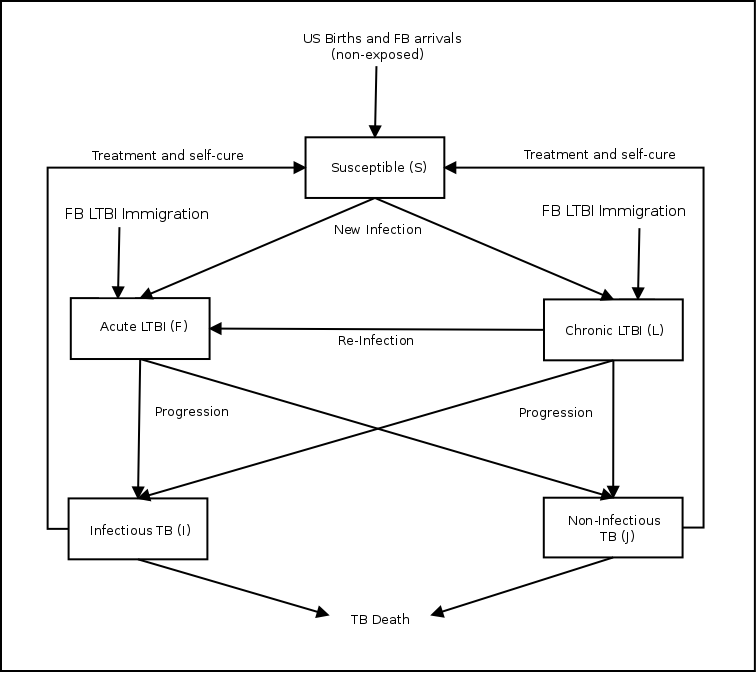
\includegraphics[scale=0.25]{figures/HillModelFlowChart.png}
  \end{center}
  \caption{Schematic of the Hill model. Each compartment represents a different
    possible TB health state for every US-born or FB individual, and arrows
    between different compartments represent possible transitions between
    states. Individuals also leave the model from all compartments due to
    natural death, which is left out of the figure for clarity. Figure adapted
    from \cite{hill_modelling_2012}}
  \label{fig:hillModelSchematic}
\end{figure}

The majority of USB and FB individuals fall into the susceptible ($S$) category,
which includes everyone who is uninfected and has not been exposed to TB, or
those who have been successfully cured of the disease. Individuals in the $S$
category flow with some rate into an LTBI category, simulating exposure to TB.
Because real LTBI patients have a higher risk of developing active TB within two
years of exposure, the Hill model splits the LTBI population among two LTBI
compartments: compartment $F$, or acute LTBI, representing those who progress
within the first two years of catching the disease, and compartment $L$, or
chronic LTBI, representing those who do not progress within the first two years.
Both LTBI compartments feed into two active TB compartments, $I$ and $J$,
representing infectious and non-infectious active TB, respectively. To respect
the varying rates of LTBI activation, individuals in the Acute LTBI compartment
have a much higher risk of developing active TB than those in the Chronic LTBI
compartment. Individuals in the Chronic LTBI compartment may also be exogenously
re-infected and transition to the Acute LTBI compartment
\cite{hill_modelling_2012}. 

Individuals in both active TB compartments have an increased risk of death from
TB infection, but only individuals in the infectious TB compartment affect the
infection flow rates. In addition, individuals in all of the infected
compartments ($F$, $L$, $I$, $J$) may be treated or self-cure themselves of
their respective TB health condition. However treatment or self-cure from TB
does not grant immunity, and all healthy individuals are grouped in the
susceptible compartment and may be re-infected at a later time
\cite{hill_modelling_2012}.

The rates that individuals move into and between compartments in the Hill model
are determined by a system of deterministic differential equations. This system
of equations, and the definitions of the constants used in the Hill model, are listed in
Appendix~\ref{appendix:hillEqs} \cite{hill_modelling_2012}. These equations
provide accurate estimations of the sizes of each compartment at any point in
time, but can provide little insight into TB dynamics beyond that, as they offer
no infection source information. Furthermore, it is important to note once again
that though real-world disease dynamics are stochastic, the Hill model is a
completely deterministic approximation and does not provide estimates for the
distributions or standard errors of predicted disease rates. We addressed each
of these issues with the extended Hill model and the agent based Hill model. 

\section{The Extended Hill Model}
\label{sec:extendHill}
In order to refine the tracking capabilities of the Hill model, the original
differential equations used to describe TB spread were separated into their
component parts and each part was tracked separately. In effect, each flow rate
between two compartments in the basic Hill model was made into its own
``virtual'' compartment, which is tracked the same as a real compartment by the
model but does not represent a particular health state. This enabled computation
not only of expected TB cases and deaths, but also the source of those cases and
deaths. A schematic for this model is shown in Figure~\ref{fig:extendedHill}.
Immigrating cases of LTBI (acute or chronic) were also tracked. In the case of
intervention testing, the number of cured and untreated cases of entering LTBI
were both tracked. 

\begin{figure}[h]
  \centering
  \includestandalone[width=\textwidth]{extendedHillFlowChart}
  \caption{A schematic of the extended Hill model. True compartments are
    illustrated in red, with flow rates illustrated with black arrows and flow
    tracking compartments illustrated in green with dashed edges.
  }
  \label{fig:extendedHill}
\end{figure}

The model was also extended to provide similarly sourced US health care system
(HCS) TB costs. To do so, we made the following treatment cost assumptions. A
single case of active TB was assumed to yield a \$14,000 US HCS cost, charged
immediately upon disease contraction. This cost is the weighted mean of the
costs of cases requiring hospitalization (49\%) and cases not requiring
hospitalization (51\%).  These cost estimates were found in \TODO{<+DYLAN COST
STUDY CITATION+>.} LTBI treatment costs were assumed to be \$468.00, charged
immediately upon successful treatment. These estimates were calculated based on
the cost of a successful treatment, and the typical adherence and efficacy of
said treatment \TODO{<+DYLAN COST STUDY CITATION, ADHERENCE CITATION+>.} Note
that active TB treatment costs are charged immediately upon disease contraction,
whereas LTBI treatment costs are charged only upon successful treatment. The
motivation for this distinction is that active TB treatment is mandated by the
US for all known cases and, further, most treatment costs are incurred at the
beginning of the treatment cycle. As such, charging for every known case,
immediately at contraction is a well motivated simplification. On the other
hand, latent TB is only rarely treated in discovered cases and the costs are
more evenly distributed. Furthermore, the choice to charge only upon successful
treatment yields a more conservative estimate of the success of any intervention
analyzed, as it will always underestimate the total US HCS TB cost burden.
Finally, it is worth noting that these estimates of US HCS treatment cost are
not intended to be fixed parameters. The code for this model is freely
available, and as new research amends the necessary costs and new methods of
treatment are developed, these values can be modified and the model re-run to
produce a revised prediction of the US HCS TB cost. In addition to US HCS cost,
the system was implemented so as to also track projected intervention
implementation cost, given user-inputted parameters relating to various possible
intervention cost strategies.  Cured cases of LTBI entering, TB deaths, total TB
cases, and total US HCS cost were also tracked discounted at 3\% annually for
cost benefit analysis. This discounting was converted to a continuous
differential equation for use within the model. 
 
The extended Hill model was implemented as a series of differential equations in
\texttt{R}, and solved using the \texttt{lsoda} system with a timestep of $0.8$.
Extensive sensitivity analysis was performed on this parameter and it was found
that decreasing the timestep did not seriously affect the model outcomes.  A
relevant subset of the extended Hill equations and a link to the full model code
and documentation can be found in Appendix~\ref{appendix:hillEqs}. Historical
data from 2000-2008 was used to initialize the model, which was then run up to
the year 2100.  

In order to understand these results statistically, a stochastic, agent based
model of TB spread in the US was implemented. This model was programmed in
\texttt{C++}, and probabilities of agent transition between various health
states were computed given rates in the hill model and a variety of integration
approximations. The model maintained individual records for every individual
with LTBI or active TB. Susceptible individuals were not modeled as agents;
instead, a binomial distribution was used to probabilistically determine the
number of new infections each time step. We ran the model with default parameter
values for 2160 runs, with time step of $0.01$.  Final population health
statistics were recorded for each run, and these data were analyzed in $R$. The
agent based model also tracks deaths, total TB cases, and infection sources.
These data were consistently normal and matched the deterministic model closely
in mean, providing statistical validation of using the deterministic model
results in intervention analysis and policy planning without more advanced
statistical analysis.

Further implementations of the agent based model were made that deviated from
the basic Hill model. Specifically, the acute latent compartment in the basic
Hill model is a vestigial necessity of compartmental modeling and is not
reflective of the biology of tuberculosis. As such, an agent based model was
implemented with one LTBI health state that relied on time-dependent
probabilities to ensure that individuals transferred within the first two years
with higher probability.  Results from this model were also normal and did not
differ significantly from the strict Hill model. This also demonstrates the
effectiveness of using agent based modeling at population level scale for
general epidemiological studies. Agent based models are much better equipped to
model population heterogeneity, drug resistance, or comorbidity, but are
typically thought to be too computationally intensive to perform on large
populations. These results show that with modern hardware, agent based modeling
can be used even with a population of millions of agents.  

\section{Results}

\subsection{Basic Population Breakdown}
The additional tracking capabilities of the extended Hill model offered several
key insights into US TB dynamics. Figure~\ref{fig:incPlotSourced} shows the
yearly incidence of US TB, broken down by infection source. Recall that
infections due to acute LTBI, in the Hill model, represent cases of a novel
infection, whereas infections due to chronic LTBI represent the activation of a
long standing latent infection.  Figure~\ref{fig:incPlotSourced} demonstrates
that the majority of the US TB load is driven by activations of FB LTBI,
followed by USB LTBI activations. Though contact investigation and aggressive TB
treatment programs help prevent increasing the LTBI population, as active TB
cases can also lead to long lasting LTBI cases, this suggests that a greater
focus on LTBI treatment would potentially have a very large impact on US TB
rates. 
\begin{figure}[h]
  \begin{center}
    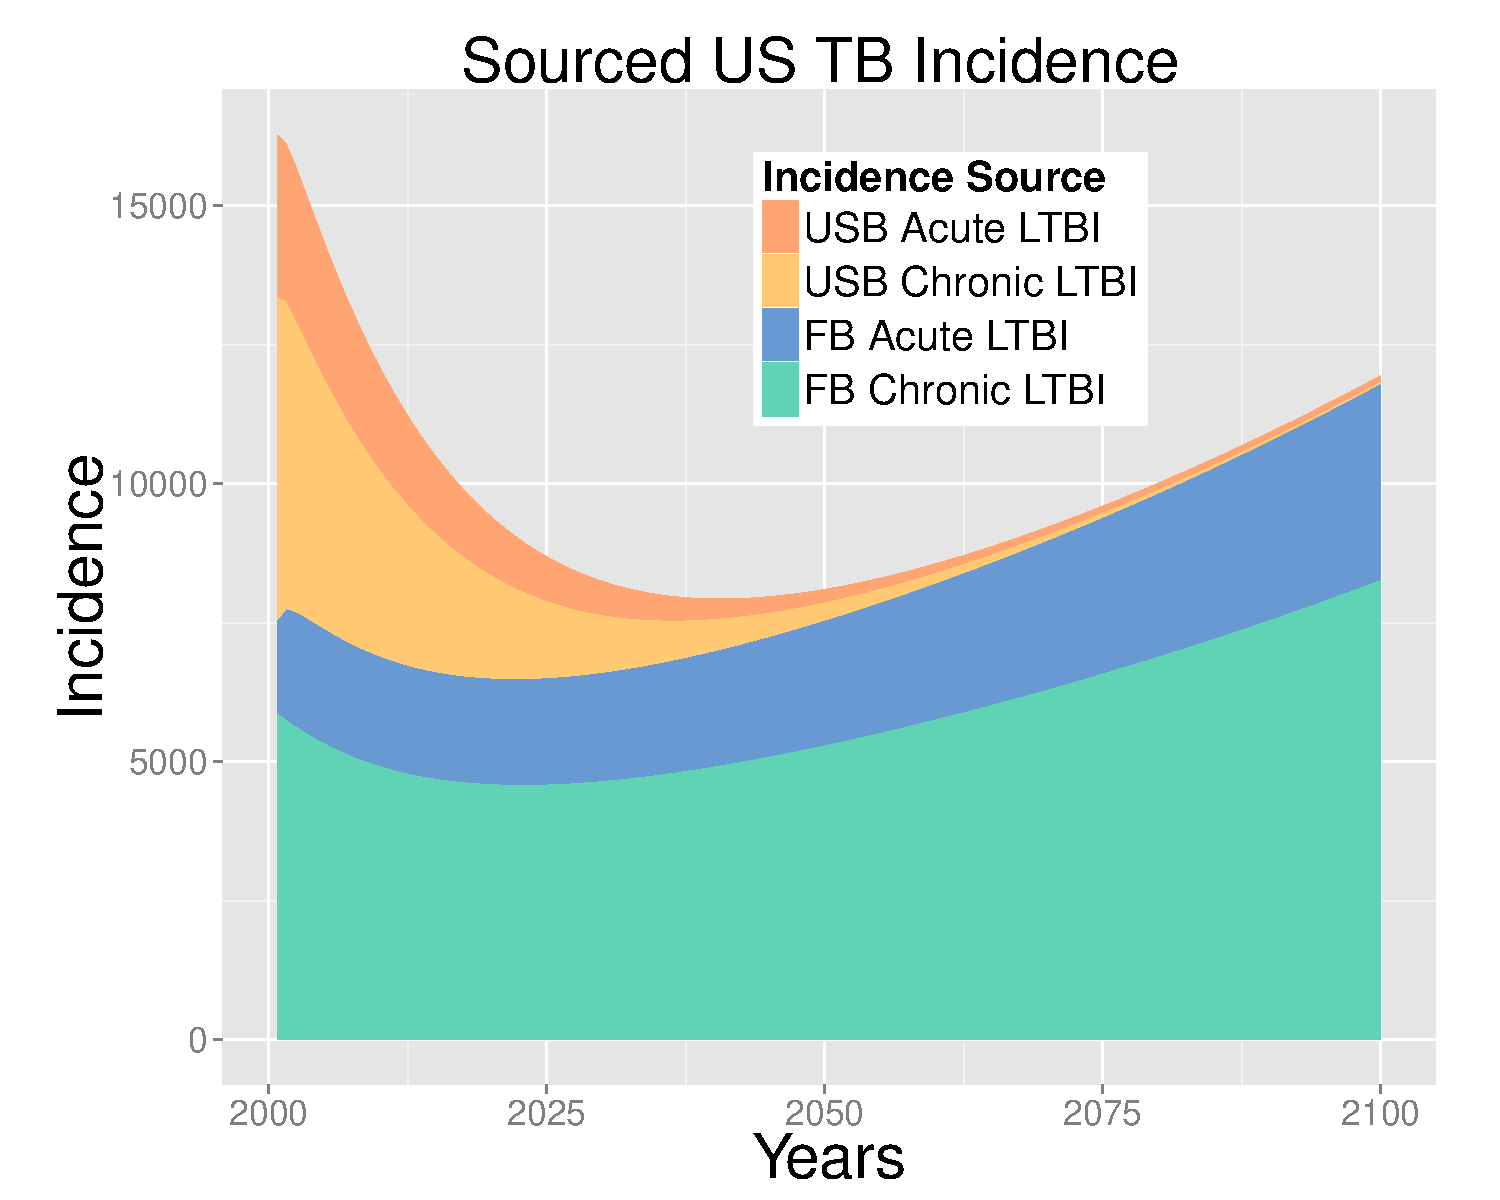
\includegraphics[scale=.5]{incPlotSourced}
  \end{center}
  \caption{Sourced yearly incidence data generated by the extended Hill model.}
  \label{fig:incPlotSourced}
\end{figure}

Figure~\ref{fig:costPlotSourced} shows a similarly sourced plot, but analyzing the
final US HCS costs due to active TB. One can see that in this plot, roughly half
of the US TB HCS costs are due to activations of LTBI. Note that, again, in this
figure it is appropriate to think of the costs due to acute LTBI as costs due to
exogenous re-inection, whereas costs due to chronic LTBI are activations of long
standing latent infections. 
\begin{figure}[h]
  \begin{center}
    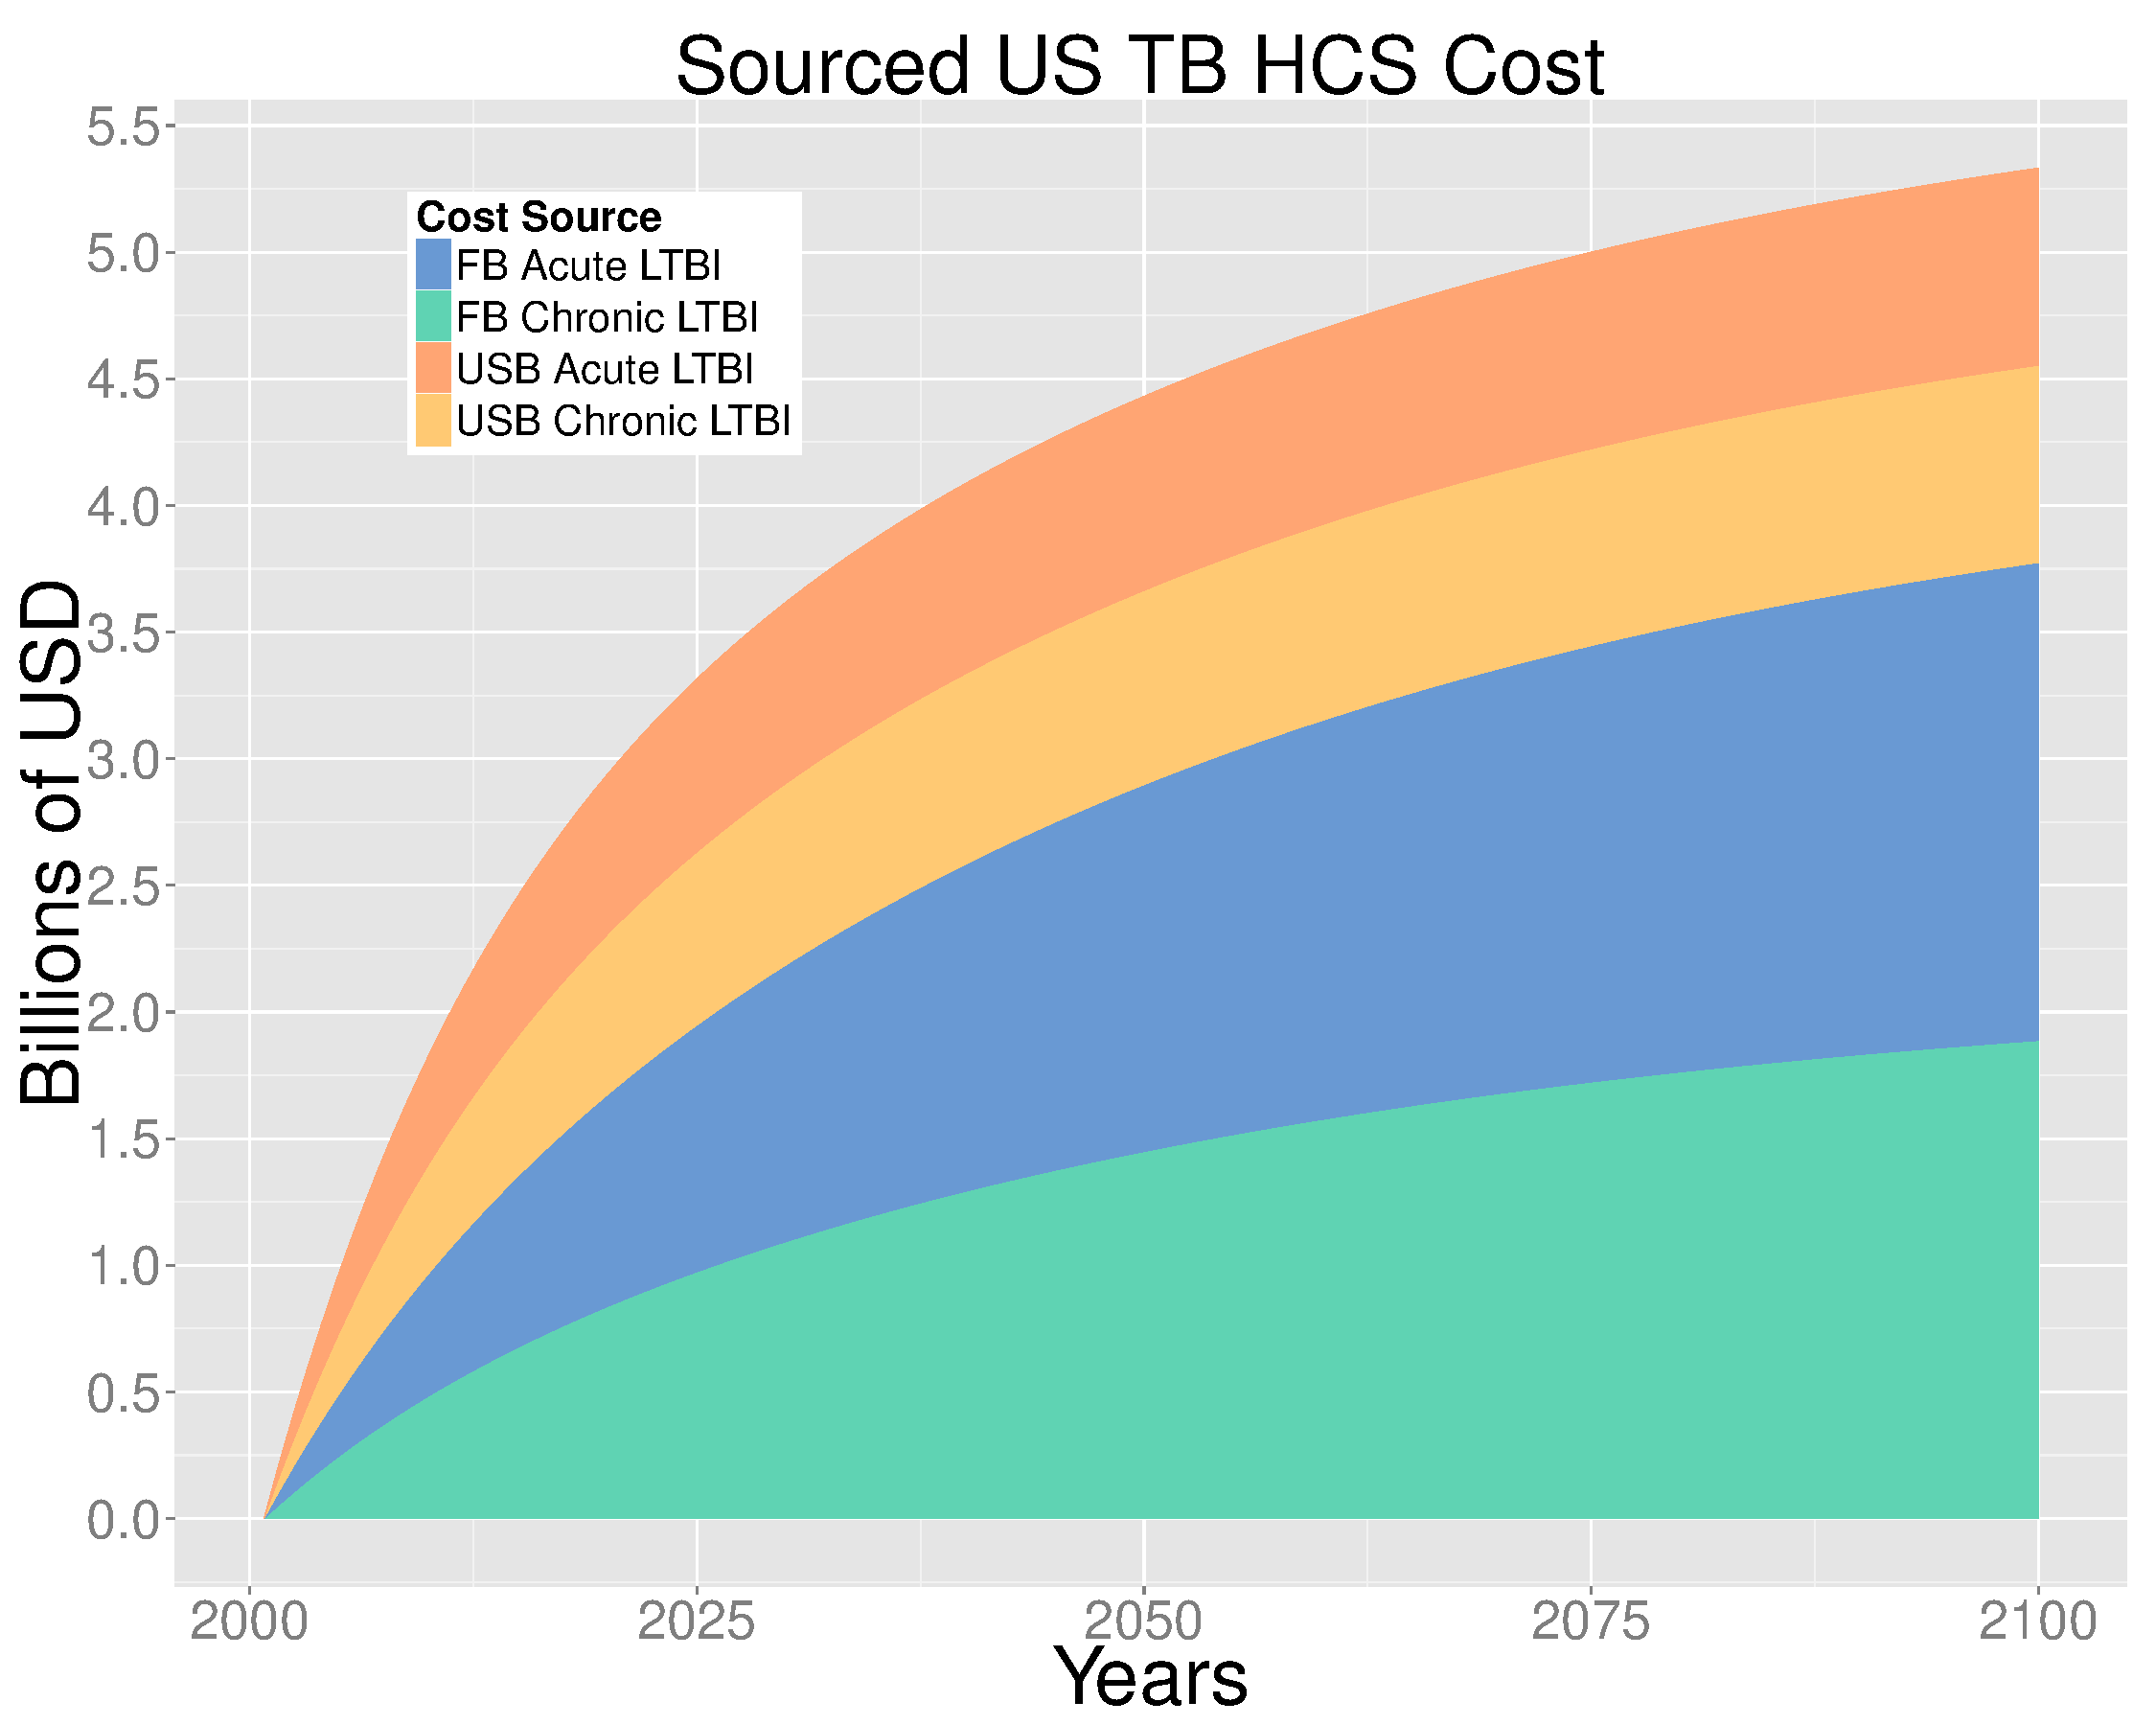
\includegraphics[scale=.35]{costPlotSourced}
  \end{center}
  \caption{Sourced US HCS economic TB load. Note that this data only illustrates
    the load due to treating active TB, but illustrates where the infections
    driving this cost come from.}
  \label{fig:costPlotSourced}
\end{figure}

In fact, both of these plots underestimate the impact of LTBI on the spread of
TB, as every chronic LTBI activation contributes not only to incidence and costs
directly, but also indirectly by causing additional future cases, which is not
captured in these graphs. Further, there are also US HCS costs due to LTBI
treatment, which are not illustrated in these graphs due to the inherent
uncertainty in estimating LTBI treatment costs. These omissions could only ever
make the case for LTBI focus stronger, as they err on the side of
underestimating its impact, not overestimating.
\subsection{Intervention Analysis}
Though the basic sourced data suggests that LTBI control may be key to US TB
control, specific intervention analysis is necessary to come to a final
conclusion, as active TB spread is potentially the driving force maintaining the
endemic LTBI population. To examine this, we tested many different
interventions, of which we will highlight two here that were particularly
noteworthy. 
\subsubsection{Curing entering LTBI cases}
As mentioned in the Introduction, the US currently tests for LTBI upon
immigration, but does not require treatment for those who test positive for LTBI
prior to admitting them entry. Given the very high TB incidence rates in certain
parts of the world, this means that the US has a very high yearly influx of LTBI
infected patients.  Curing these patients of LTBI upon entry represents an
excellent strategy of targeting the LTBI population because it is requires
effectively no cost to find those infected with LTBI. As those with LTBI are
asymptomatic, normally LTBI treatment is hindered by the fact that seeking out
those with LTBI can be quite costly. However, here, the process of finding those
with LTBI is already performed, so the question is only one of the benefits and
costs of the treatment alone. To assess this intervention, we ran the model for
various entering LTBI cure rates. Figure~\ref{fig:redEnLTBIInc} shows these
results for $10\%$, $25\%$, $50\%$, and $100\%$ entering LTBI cure rate. 
\begin{figure}[h]
  \centering
  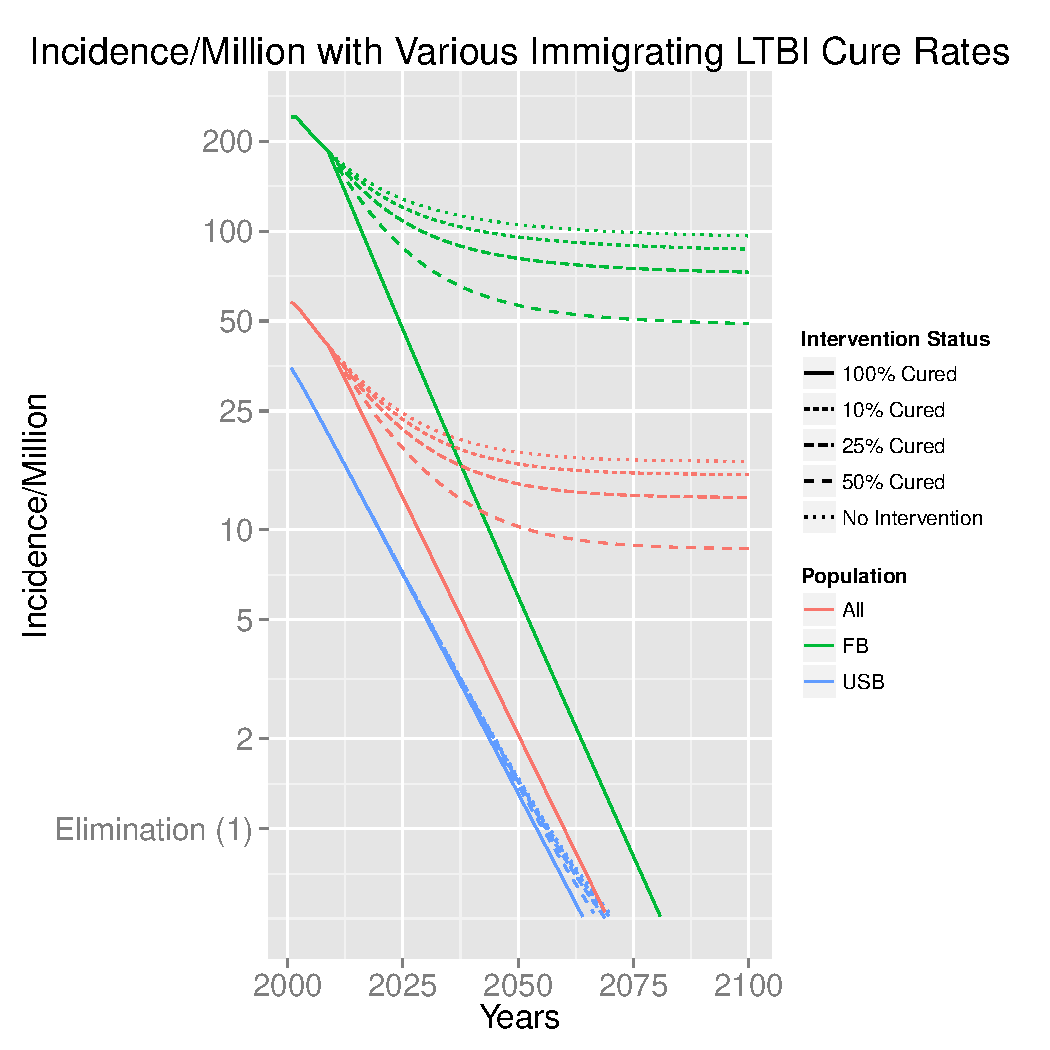
\includegraphics[width=0.8\textwidth]{figures/redEnLTBI}
  \caption{The resulting incidence per million given various levels of entering
    LTBI cure rates.}
  \label{fig:redEnLTBIInc}
\end{figure}

Note that the Extended Hill model does not differentiate between documented and
undocumented immigration, so these percentages of cases cured include curing
cases of undocumented immigration, despite that the fact that they are not
tested for LTBI in the first place, as a result of their unofficial channel of
entry. Thus, achieving 100\% entering LTBI cure rates is practically impossible;
however, it does illustrate a very important result.  Note that both other
tested cure rates predict that eventually, incidence rates plateau, reaching a
nearly steady state by 2075.  This plateau indicates that the system has reached
an endemic state, where TB lives on in the population despite intervention
efforts. Given the United States' already aggressive treatment of active TB, why
does this plateau occur?  Our new model concretely demonstrates that this
plateau occurs exactly because the US maintains a sizable influx into its LTBI
population due to immigration, constantly maintaining the population at a large
enough level to ensure consistent activations of active TB. If the LTBI
population does not decay, then an endemic state will always be the final
solution, as regardless of how aggressively active TB is treated, the
asymptomatic LTBI population will always produce new cases. In our studies,
every intervention observed had this plateauing effect, save reducing entering
LTBI by 100\%. This establishes that it is precisely the constantly replenishing
LTBI population that maintains US TB incidence. To demonstrate this more
concretely, we consider another intervention, one which will isolate the effects
of the LTBI driven TB dynamics versus the spread of active TB in all its forms. 

\subsubsection{Eliminating TB transmission}
We also analyzed the intervention of eliminating all active TB transmission. In
other words, after the start of the intervention, all TB spread is simply
stopped; everyone infected with TB is noninfectious. This simply removes any
real dependence on active TB spread, and instead highlights the incidence that
stems from the self-replenishing LTBI population alone.
Figure~\ref{fig:redTrans100} demonstrates this effect. 
\begin{figure}[h]
  \centering
  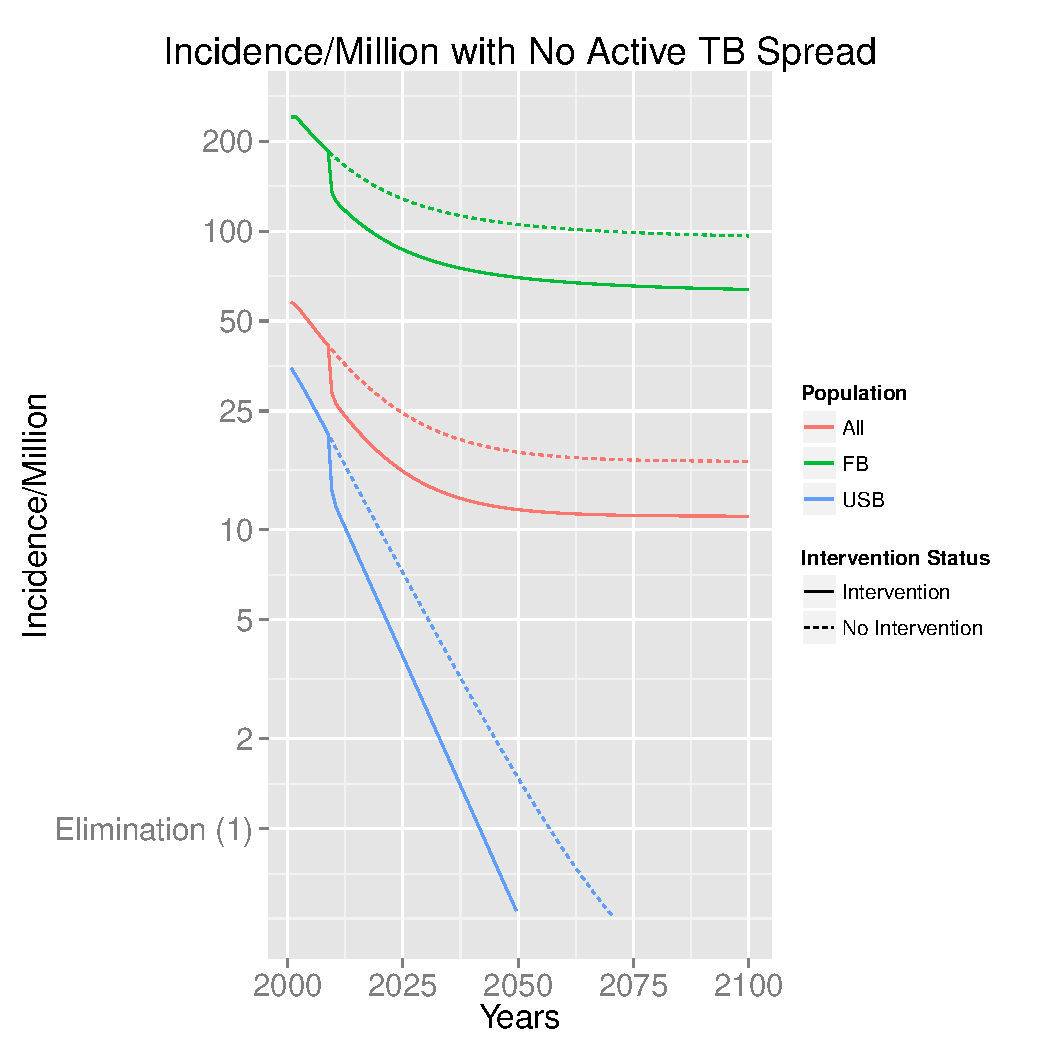
\includegraphics[width=0.8\textwidth,page=1]{figures/redTrans100Analysis}
  \caption{This figure shows the yearly TB incidence per million given either no
  intervention or eliminating active TB transmission.}
  \label{fig:redTrans100}
\end{figure}

Figure~\ref{fig:redTrans100} demonstrates that eliminating active TB
transmission is only moderately effective and still maintains the plateauing
effect. Therefore, this endemic state is entirely due to the LTBI population. As
it is substantially higher than the US goal for elimination, this demonstrates
that LTBI treatment is essential to reach elimination by 2100. Among all LTBI
treatment interventions tested, curing entering cases of LTBI was the most
effective by far, for the reasons outlined above. Unfortunately, in order to
obtain elimination by 2100, at least 95\% of entering LTBI cases had to
be cured, which is realistically infeasible. Note that sensitivity analysis
results also indicated that cure rates for entering LTBI cases and LTBI
treatment rates were highly influential parameters, both in the US HCS costs and
in the number of active infections. 

\subsubsection{Cost Effectiveness}
\TODO{It also needs to talk about the cost effectiveness of reducing
  transmission or something, to say that we're getting competitive numbers. We
need a good source for cpca data for contact investigations, etc.}
We also estimated the cost per case averted of curing entering cases of LTBI. To
do so, we assumed that curing a single case of entering LTBI would cost \$800.
This number is substantially higher than the assumed domestic LTBI treatment
cost for a number of reasons; notably the cost of implementation as part of the
immigration process would be very nontrivial. However, this inflation is also
meant to be a conservative estimate, so as to underestimate the effectiveness of
this intervention rather than overestimate. Given this treatment cost, we found
that curing 25\% of entering cases of LTBI resulted in a net US HCS cost per
case averted of \$67,654.07 at 2025, \$28,699.15 at 2050, and
\$17,912.95 at 2100 (see Table \ref{tab:redEnLTBICosts} for the cost per case
averted for other cure percentages). Given the variable nature of LTBI treatment
cost, the model code is built so that a user can adjust these costs themselves
to explore more specific methods of curing entering LTBI, especially as the
treatment methods and associated costs evolve in future years. Curing
immigrating cases of LTBI  also resulted in 11,900, 29,880, and 60,189 fewer
cases of TB and 1,025, 2,573, and 5,185 fewer TB deaths for 10\%, 25\%, and 50\%
cure rate, respectively.

%We also found that the relationship between total incidence at 2100 and
%percentage of incoming LTBI cases cured was linear. Given this, we estimated the
%yearly average US HCS savings garnered by curing one case of entering LTBI per
%year from 2000 to 2025, 2000 to 2050, and 2000 to 2100.  This value peaked
%at \$1.283 billion at 2100 (25\% reduction). This illustrates that it
%would be cost saving to cure cases of LTBI at the cost of \$1.283 billion
%``2000'' dollars over the time period 2000-2100. 
%These findings are illustrated in Table~\ref{tab:redEnLTBICosts}

\begin{table}
\centering
\begin{tabular}{|r|cccc|} \hline
      &5\% Reduction&10\% Reduction&25\% Reduction&50\% Reduction\\\hline
  2025& \$67,908.81 & \$67,855.46 & \$67,654.07 & \$67,332.53 \\ 
  2050& \$28,938.23 & \$28,878.70 & \$28,699.15 & \$28,404.13 \\ 
  2075& \$21,044.88 & \$20,989.16 & \$20,820.53 & \$20,541.77 \\ 
  2100& \$18,130.11 & \$18,076.11 & \$17,912.95 & \$17,642.64 \\ \hline
\end{tabular}
\caption{Cost Per Case Averted by Reducing Incoming LTBI by various percentages
(in dollars per case)} 
\label{tab:redEnLTBICosts}
\end{table}

\subsection{Agent Based Evaluation}
Though the extended Hill model is validated against both the Hill model and real
world data for the years 2000-2008, it still lacks the ability to describe the
statistical parameters underlying its results. Real disease spread is
stochastic, yet from the extended Hill model alone we do not know what
distribution the final infection counts will take. The agent-based model allowed
these statistical properties to be analyzed and thus gave us confidence in the
statistical reliability of the extended Hill results. In particular, it
illustrated that the deterministic Hill model provides a robust statistical
measure of TB epidemic behavior in the US conditions, as we found that the
distribution of incidence and final population sizes were approximately
normal, with mean accurate to the deterministic model and very tight standard
deviations. Figure~\ref{fig:finalDists} shows the final distributions for a run
of approximately 2100 iterations of the agent based model. 
\begin{figure}[h]
  \centering
  \begin{minipage}{0.45\textwidth}
    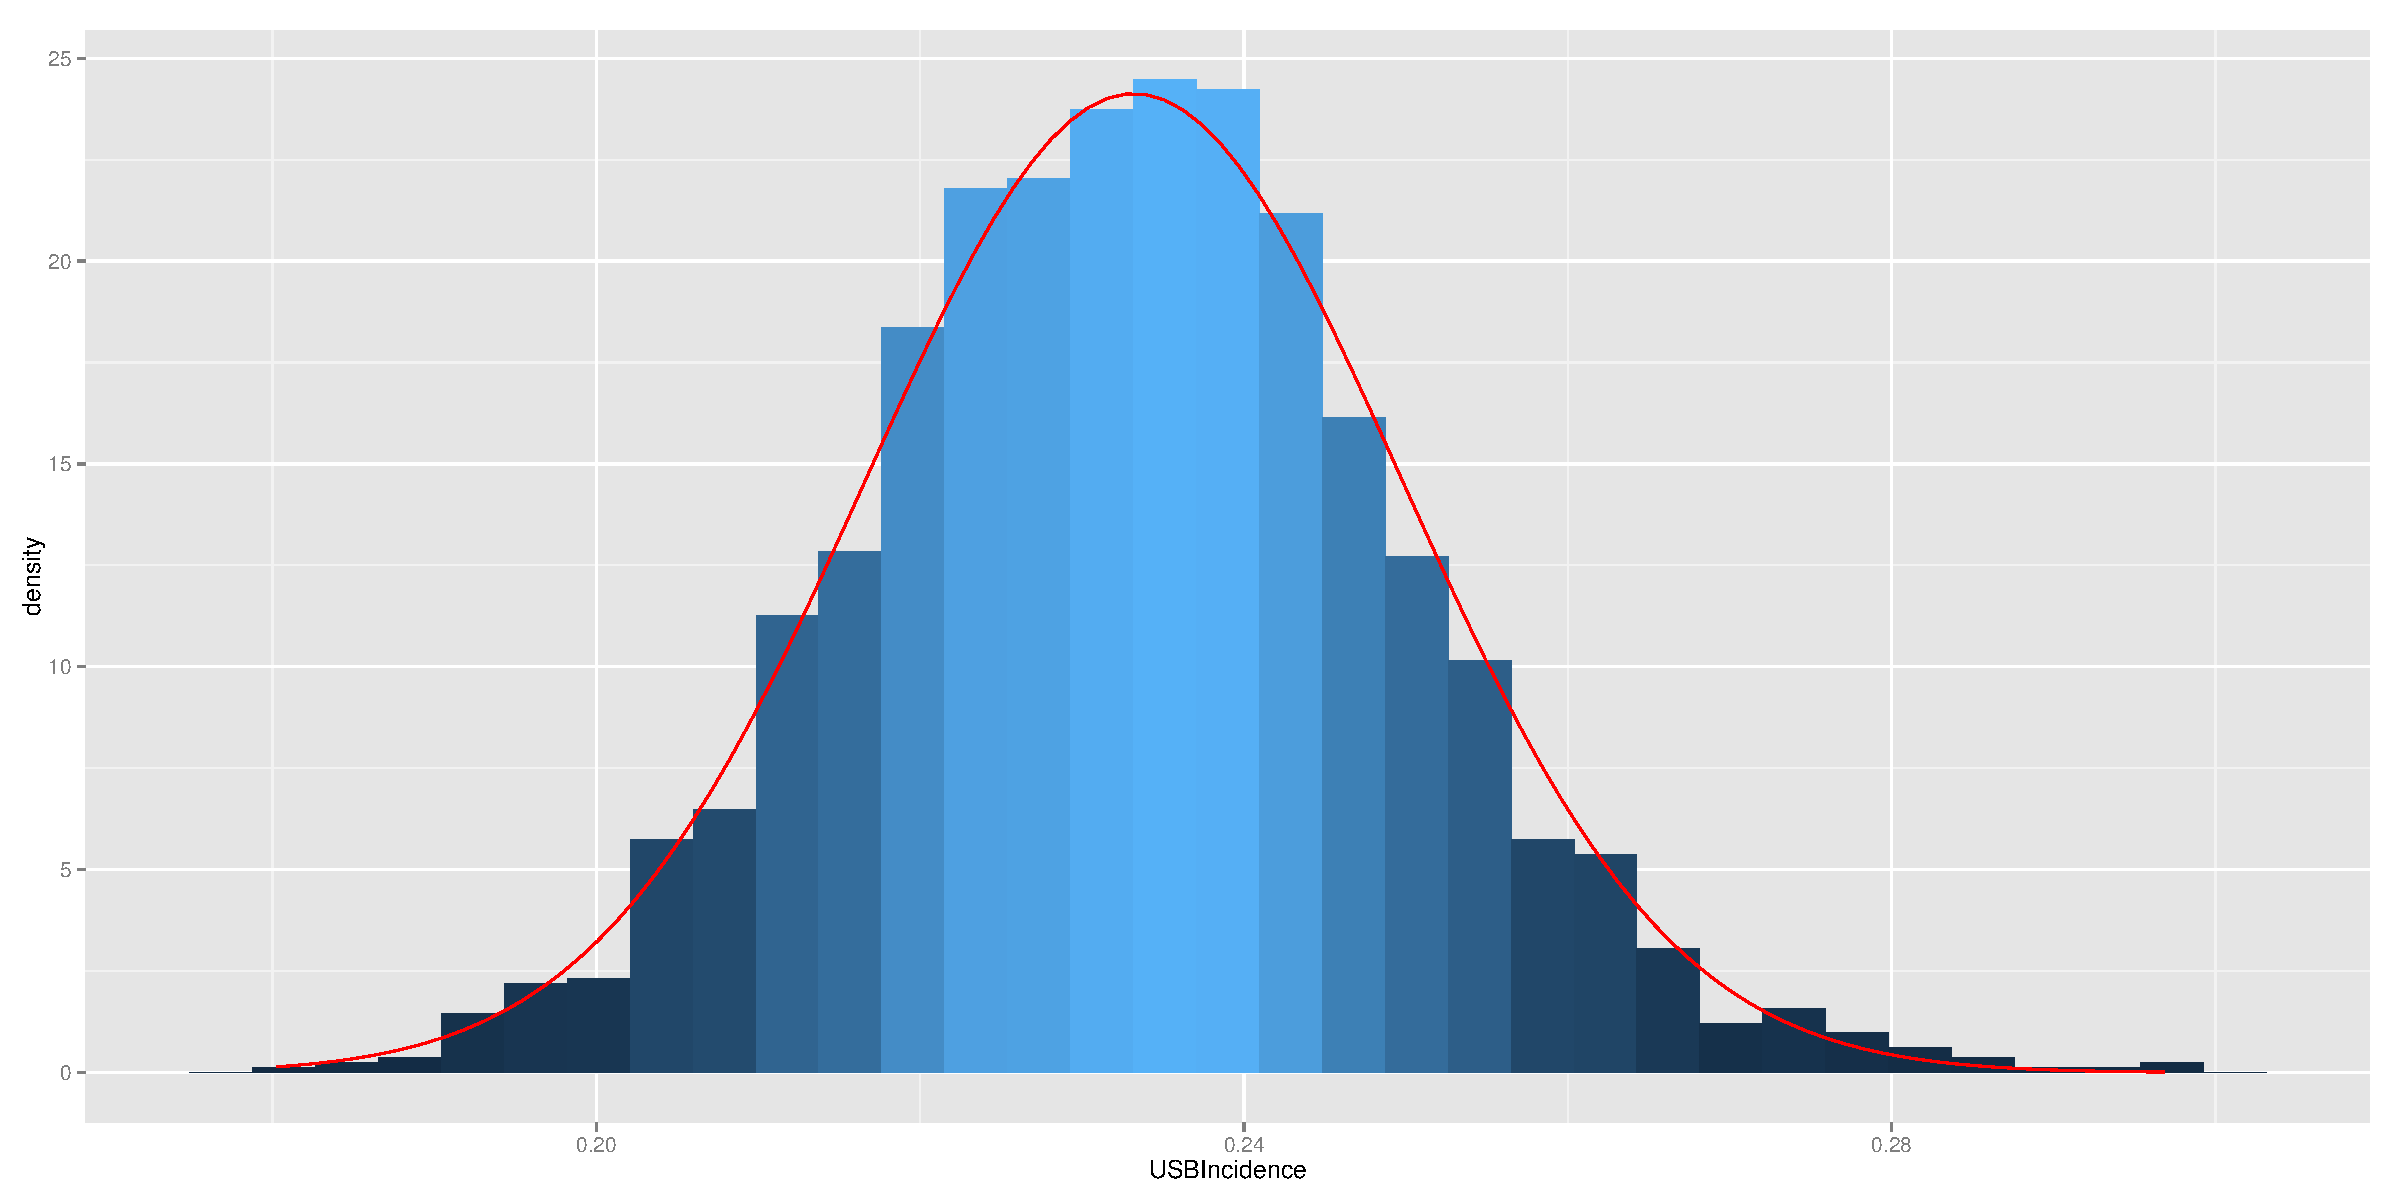
\includegraphics[width=0.95\textwidth]{figures/IN0distOrig}
  \end{minipage}
  \begin{minipage}{0.45\textwidth}
    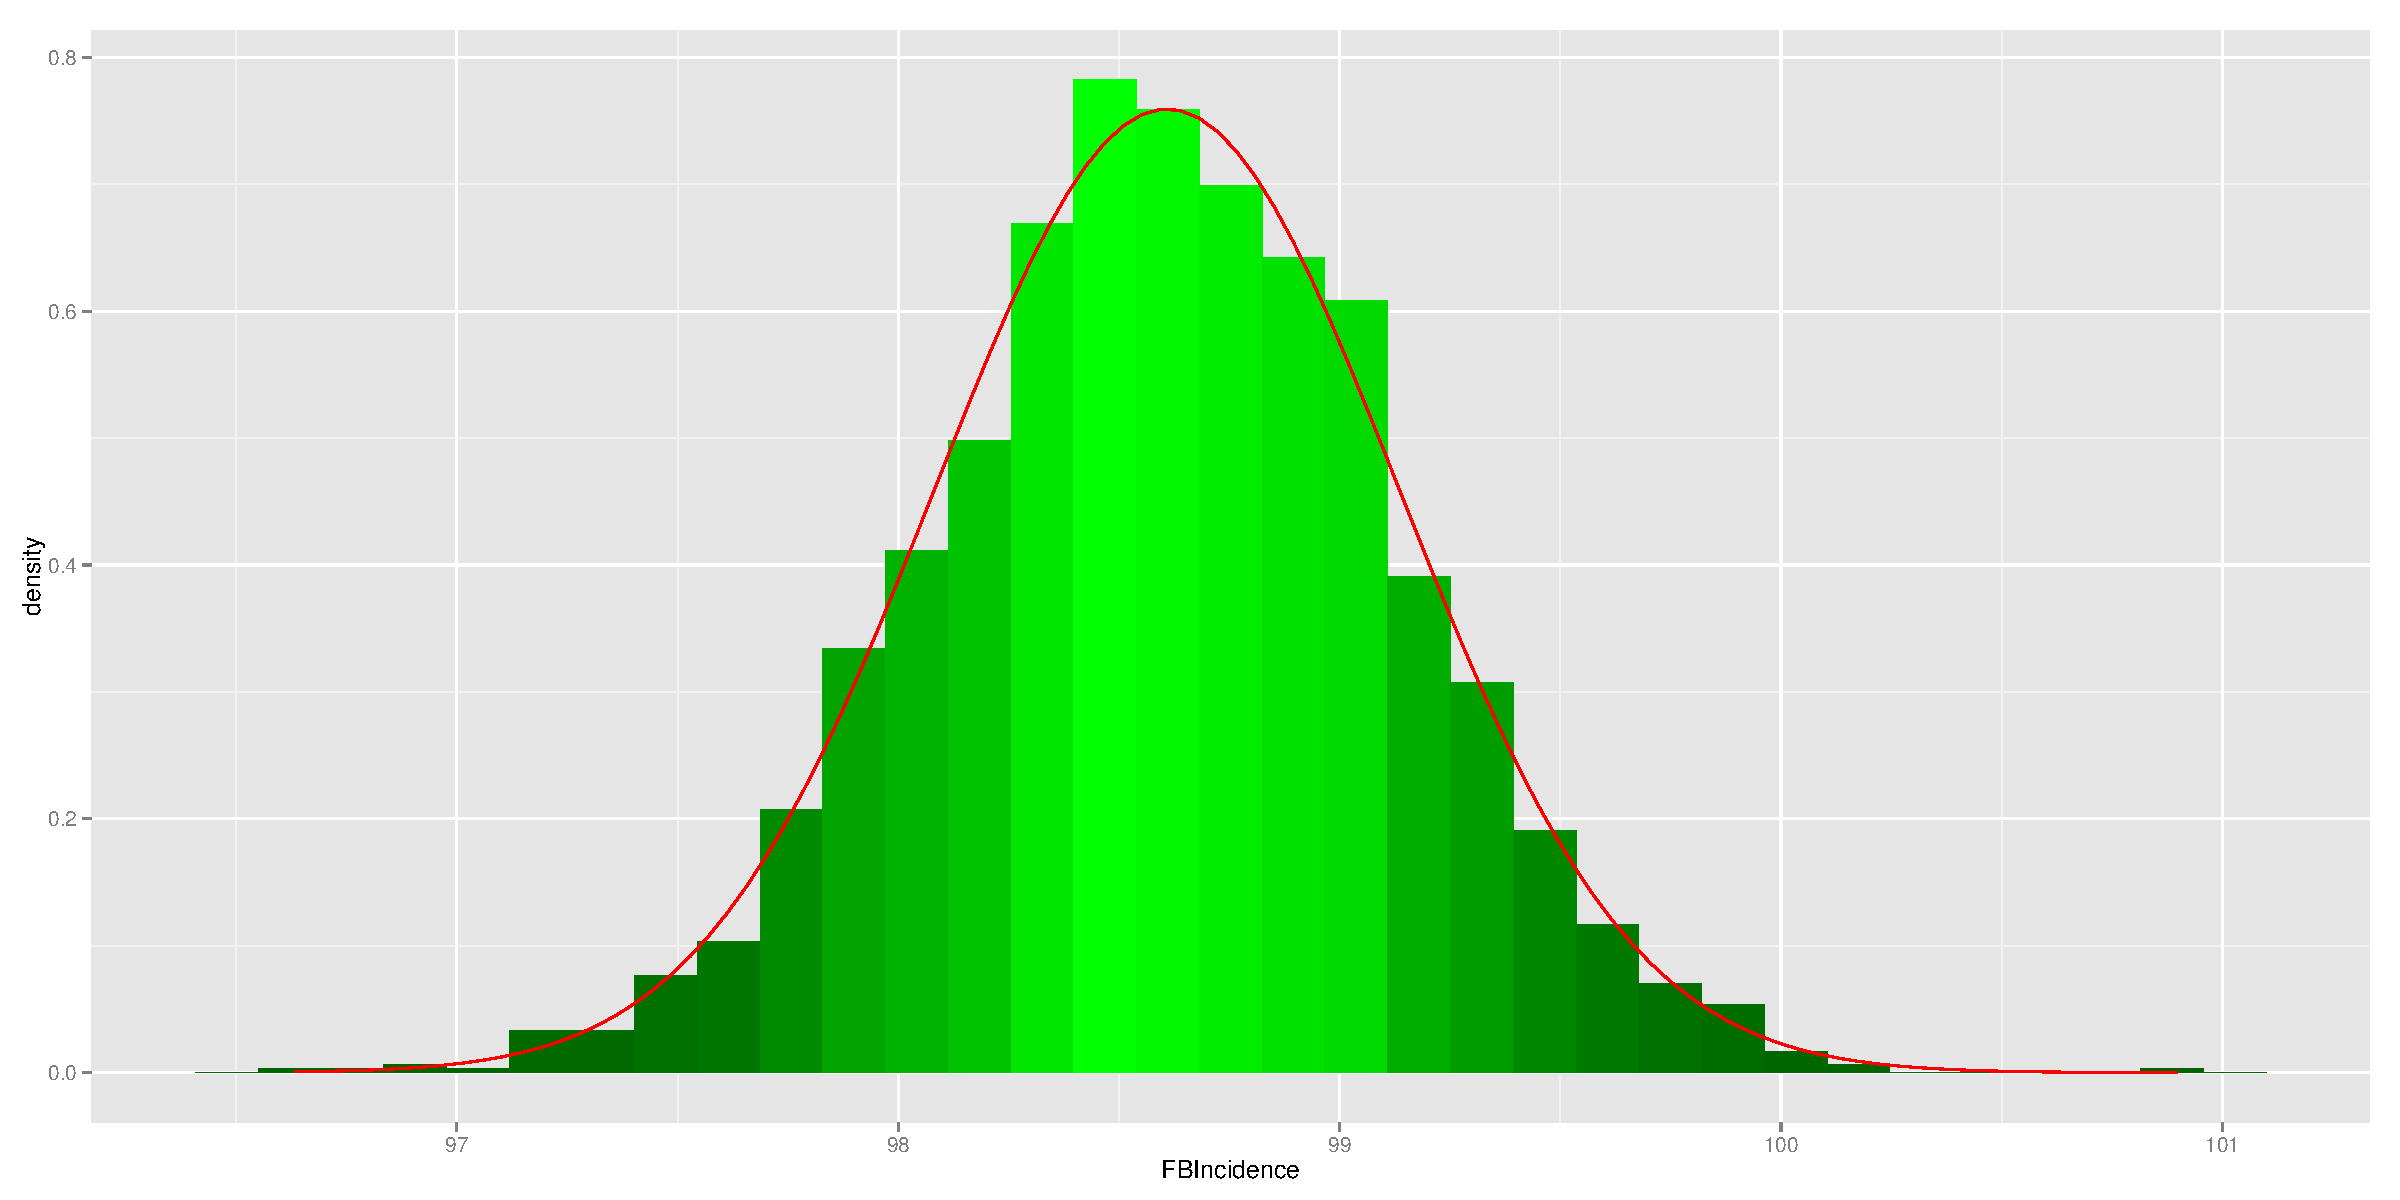
\includegraphics[width=0.95\textwidth]{figures/IN1distOrig}
  \end{minipage}
  \caption{This figure shows the final distributions (at 2100) for the USB
    incidence per million \textit{(left)} and FB incidence per million
    \textit{(right)}. The data were approximately normal, with parameters given
    by $\mu = 0.233$, $\sigma = 0.016534$, and $\mu = 98.6$, $\sigma = 0.525294$
    for the USB and FB incidence levels, respectively. The hill model predicts
    final incidence levels of $0.231$ and $96.36$, respectively, so these match
    quite well given they come from different model frameworks.
  }
  \label{fig:finalDists}
\end{figure}

Additionally, the agent-based model provided a computational
framework to produce meaningful intervention results. On student lab grade
hardware, a statistically meaningful experiment could be run overnight,
producing data in one day. This demonstrates that this modeling strategy is
feasible in this general case.  Furthermore, the agent-based model provides a
greater extensibility to more specific and biologically reasonable scenarios,
such as geographic dependency or greater population heterogeneity.  

\section{Conclusion}
These results suggest that  LTBI treatment is essential to
controlling US TB dynamics. This is demonstrated through current US TB incidence
sources as well as specific intervention analysis. 
Furthermore, our model indicates that without an active effort to treat
entering cases of LTBI, the US is likely to never reach its elimination goal, due to the plateauing
effect. To attain elimination of TB in the US by 2100, we need to cure approximately
95\% of entering LTBI cases per year, though this number may be reduced if
combined with other, LTBI targeting interventions. 

In addition to immigrant LTBI treatment programs, the US government may consider
investing in foreign TB control programs, to help bring TB incidence down
globally so that our LTBI influx rate naturally slows. Further analysis
incorporating immigration source (i.e. country of origin) and regional TB
dynamics in the US would be able to determine which foreign TB programs would
most warrant domestic aid. This would be a natural extension of this work,
which could help guide US TB policy after implementing domestic interventions.  

The agent based model may also be extended to account for greater population
heterogeneity, tracking more health parameters for each individual.
Parameters such as HIV infection status, geographic location, and multi-drug
resistant TB could be added to yield additional information about TB disease dynamics.
For agent based models, simulation run times scale linearly with the number of health
states, as opposed to exponentially for compartment based models. Therefore,
these extensions could be made without significant increases in computational power.

\section{Appendix} 
\subsection{The Hill Model}
\label{appendix:hillEqs}
The differential equations governing the basic Hill model, which also govern the overall compartment flow
in the extended Hill model, are shown in Figure~\ref{fig:hillEquations}, while
the constants governing these equations are shown in
Figure~\ref{fig:hillConstants}. In these equations, note that the variables
$S_0, F_0, L_0, I_0, J_0$ contain the number of US-born individuals in the $S$,
$F$, $L$, $I$, $J$ compartments respectively, whereas $S_1, F_1, L_1, I_1, J_1$
contain the number of foreign-born individuals. $N_0$ and $N_1$ are the total
populations of US-born and foreign-born individuals \cite{hill_modelling_2012}.
\begin{figure}[h]
  \begin{align*}
    \dot{S}_0 &= \rho(N_0+N_1) + \sigma_0^FF_0 + \sigma^LL_0 
                +\varphi_0(I_0+J_0) - \lambda_0 S_0 - \mu_0 S_0\\
    \dot{F}_0 &= p\lambda_0S_0 + xp\lambda_0L_0 - (\mu_0+\nu^F+\sigma_0^F)F_0\\
    \dot{L}_0 &= (1-p)\lambda_0S_0 - xp\lambda_0L_0 
                -(\mu_0+\nu_0^L+\sigma^L)L_0\\
    \dot{I}_0 &= q(\nu^FF_0 + \nu_0^LL_0) - (\mu_0+\mu^d+\varphi_0)I_0\\
    \dot{J}_0 &= (1-q)(\nu^FF_0 + \nu_0^LL_0) - (\mu_0+\mu^d+\varphi_0)J_0\\
    \dot{S}_1 &= (1-f)\alpha(N_0+N_1) + \sigma_1^FF_1 + \sigma^LL_1 
                +\varphi_1(I_1+J_1) - \lambda_1S_1 - \mu_1S_1\\
    \dot{F}_1 &= gpf\alpha(N_0+N_1) + p\lambda_1S_1 + xp\lambda_1L_1 
                -(\mu_1+\nu^F+\sigma_1^F)F_1\\
    \dot{L}_1 &= (1-gp)f\alpha(N_0+N_1) + (1-p)\lambda_1S_1 - xp\lambda_1L_1 
                -(\mu_1+\nu_1^L+\sigma^L)L_1\\
    \dot{I}_1 &= q(\nu^FF_1 + \nu_1^LL_1) - (\mu_1+\mu^d+\varphi_1)I_1\\
    \dot{J}_1 &= (1-q)(\nu^FF_1 + \nu_1^LL_1) - (\mu_1+\mu^d+\varphi_1)J_1\\
  \end{align*}
  \caption{System of Differential Equations given in the Hill model.}
  \label{fig:hillEquations}
\end{figure}
\begin{figure}[h]
  \begin{align*}
    \rho       &= 0.018   && \text{(US birth rate)}\\
    \alpha     &= 0.005   && \text{(FB arrival rate)}\\
    \mu_0      &= 1/78    && \text{(Natural USB mortality rate)}\\
    \mu_1      &= 1/53    && \text{(FB mortality rate)}\\
    \sigma^{L} &= 0.057   &&\text{(Treatment rate for chronic LTBI)}\\
    \nu^{L}_{0}&= 0.0014  &&\text{(Progression rate for reactivation in the USB
                                   population)}\\
    \nu^{L}_{1}&= 0.0010  &&\text{(Progression rate for reactivation in the FB
                                   population)}\\
    \nu^{F}    &= 1.5     &&\text{(Progression rate for acute LTBI)}\\
    f          &= 0.187   &&\text{(Fraction of FB arrivals with LTBI)}\\
    p          &= 0.103   &&\text{(Fraction of new infections which are acute)}\\
    ARI_{0}    &= 0.00030 &&\text{(2000 Annual Risk of Infection, USB)}\\
    q          &= 0.708   &&\text{(Fraction of infections progressing to infectious
                                   disease)}\\
    g          &= 0.0047  &&\text{(Fraction of FB arrivals with LTBI who are fast
                                   progressors)}\\
    \sigma^{F} &= 0.461   &&\text{(Cumulative fraction of treatment for acute
                                   infection)}\\
    \sigma_0^{F} &= 1.296 &&\text{(Rate of treatment for USB acute infection)}\\
    \sigma_1^{F} &= 1.301 &&\text{(Rate of treatment for FB acute infection (per
                                   year))}\\
    r_{0}      &= 0.667   &&\text{(Fraction of cases due to reactivation in USB
                                   population)}\\
    r_{1}      &= 0.780   &&\text{(Fraction of cases due to reactivation in FB
                                   population)}\\
    \mu^{d}    &= 0.115   &&\text{(Mortality rate due to TB)}\\
    x          &= 0.111   &&\text{(Fraction of re-infected chronic LTBI moving to
                                   acute infection)}\\
    \phi       &= 0.897   &&\text{(Cumulative fraction self-cure and treatment of
                                   active disease)}\\
    \phi_0     &= 0.897   &&\text{(Cumulative rate of self-cure and treatment of
                                   USB active disease)}\\
    \phi_1     &= 0.897   &&\text{(Cumulative rate of self-cure and treatment of
                                   FB active disease)}\\
  \end{align*}
  \begin{align*}
    e_{0}      &= 0.965   &&\text{(Fraction of intra-USB preferred contacts)}\\
    e_{1}      &= 0.985   &&\text{(Fraction of intra-FB preferred contacts)}\\
    \beta      &= 10.39   && \text{(Effective contact rate)}\\
    \lambda_i  &= \beta\(c_i0\frac{I_0}{N_0} + c_{i1}\frac{I_1}{N_1}\)
                          &&\text{(The force of infection)}\\
    c_{ij}     &= e_i\delta_{ij} + (1-e_i)\frac{(1-e_j)N_j}
                                               {(1-e_0)N_0 + (1-e_1)N_1}
                          &&\text{(Contact proportion constants)}\\
  \end{align*}
  \caption{The relevant constants used in the basic Hill model. All rates are in
           units of year$^{-1}$.}
  \label{fig:hillConstants}
\end{figure}

As mentioned above, the equations shown in Figure~\ref{fig:hillEquations} govern
both the basic Hill model and the extended Hill model; the difference between
the two is that in the extended Hill model, the equations were separated into
their component parts so that each flow rate could be captured individually. For
example, the equation
\[\dot{I}_0 = q(\nu^FF_0 + \nu_0^LL_0) - (\mu_0+\mu^d+\varphi_0)I_0\]
was separated into 
\begin{align*}
  \dot{{I_0}}_{F_0} &= q \nu^F F_0\\
  \dot{{I_0}}_{L_0} &= q \nu_0^L L_0\\
  \dot{{TBD}}_{I_0} &= \mu^dI_0 \\
  \dot{{ND}}_{I_0}  &= \mu_0I_0 \\
  \dot{{S}}_{I_0}   &= \varphi_0 I_0\\
  \dot{I_0}         &= \dot{{I_0}_{F_0}} + \dot{{I_0}_{L_0}} +
                       \dot{{TBD}_{I_0}} - \dot{{TBD}_{I_0}} -
                       \dot{{ND}_{I_0}}  - \dot{S_{I_0}}
\end{align*}
where ${I_0}_{F_0}$ is the number of USB active, contagious infections (members
of $I_0$) that arose due to new infections (activations from the USB acute LTBI
compartment, $F_0$), ${I_0}_{L_0}$ is the number of USB active infections that
arose from activations of longstanding LTBI infections (the USB chronic LTBI
compartment, $L_0$), ${TBD}_{I_0}$ is the number of TB deaths from those in the
infectious USB population, $I_0$, $ND_{I_0}$ is the number of natural deaths
from those in the infectious USB population, and $S_{I_0}$ is the number of
cases of active, infectious TB in the USB population that were cured. 

The extended Hill also added certain equations and constants to generate cost
data. These equations are detailed in Figure~%\ref{fig:hillCosts}. 
\TODO{Add figure hillCosts. We first need to determine what the correct LTBI
cost parameters are. See the TODO above regarding that.}
These parameters were derived via
\TODO{Cite Dylan's cost study, adherence study, etc.}

Finally, all the code for the extended hill and agent based model can be found
on github, at \url{https://github.com/mmcdermott/disease-modeling}.

\newpage
\bibliographystyle{plain}
\bibliography{draft}
\end{document}
